\subsection{Эллипс}
\textit{Эллипс} --- плоская замкнутая кривая, сумма расстояний от любой точки котрой до двух фиксированных точек, называемых фокусами, постоянна и равна удвоенной большой полуоси эллипса.
\begin{equation}F_1M+F_2M=const=2a
\end{equation}
Главные отрезки эллипса:

1. \textit{Большая полуось} ($a $)
2. \textit{Малая полуось } ($b $)
3. \textit{Фокусное расстояние } ($c $)

$a$, $b$ и $c$ связаны следующим образом: $b^2+c^2=a^2$, что несложно вывести из определения эллипса.
 Эксцентриситет ($e$) --- числовая характеристика, показывающая степень отклонения от окружности. В эллипсе $0<e<1$.
 \begin{center}
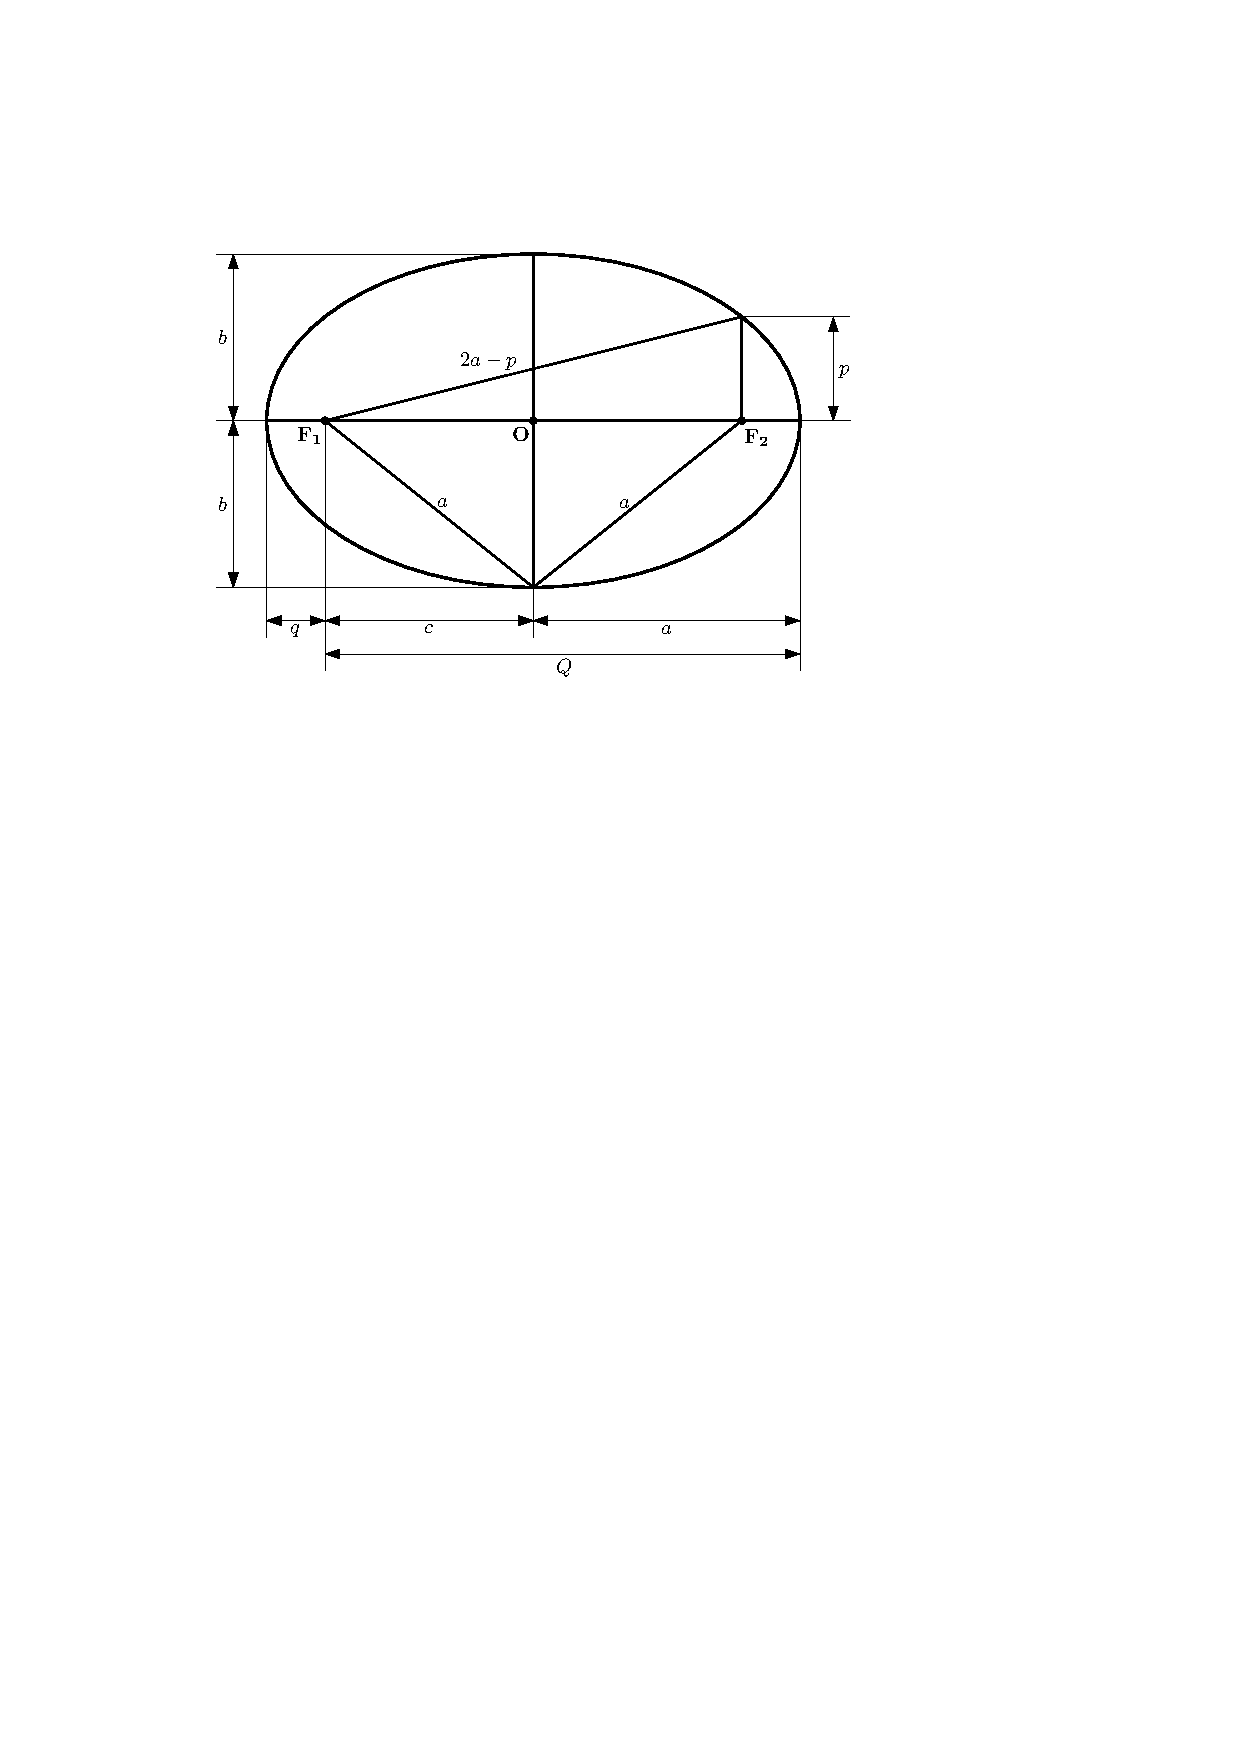
\includegraphics[width = 0.8\textwidth]{Ellips}
\begin{figure}[h!]
\caption{Эллипс}
\end{figure}
\end{center}
\paragraph{Основные формулы для эллипса}

\begin{flushleft}
Эксцетриситет
\end{flushleft}
\begin{equation}
e=\frac{c}{a}=\sqrt{1-\frac{b^2}{a^2}}
\end{equation}
Расстояние до апоцентра
\begin{equation}
Q=a(1+e)
\end{equation}
Расстояние до перицентра
\begin{equation}
q=a(1-e)
\end{equation}
Фокальный параметр
\begin{equation}
p=\frac{b^2}{a}=a(1-e^2)=b\sqrt{1-e^2}
\end{equation}
Площадь эллипса
\begin{equation}
S=\pi ab
\end{equation}

Радиус кривизны дуги эллипса в зависимости от расстояния $x$ от фокуса:
\begin{equation}
R=\frac{(2ax-x^2)^{3/2}}{ab}
\end{equation}
\begin{center}
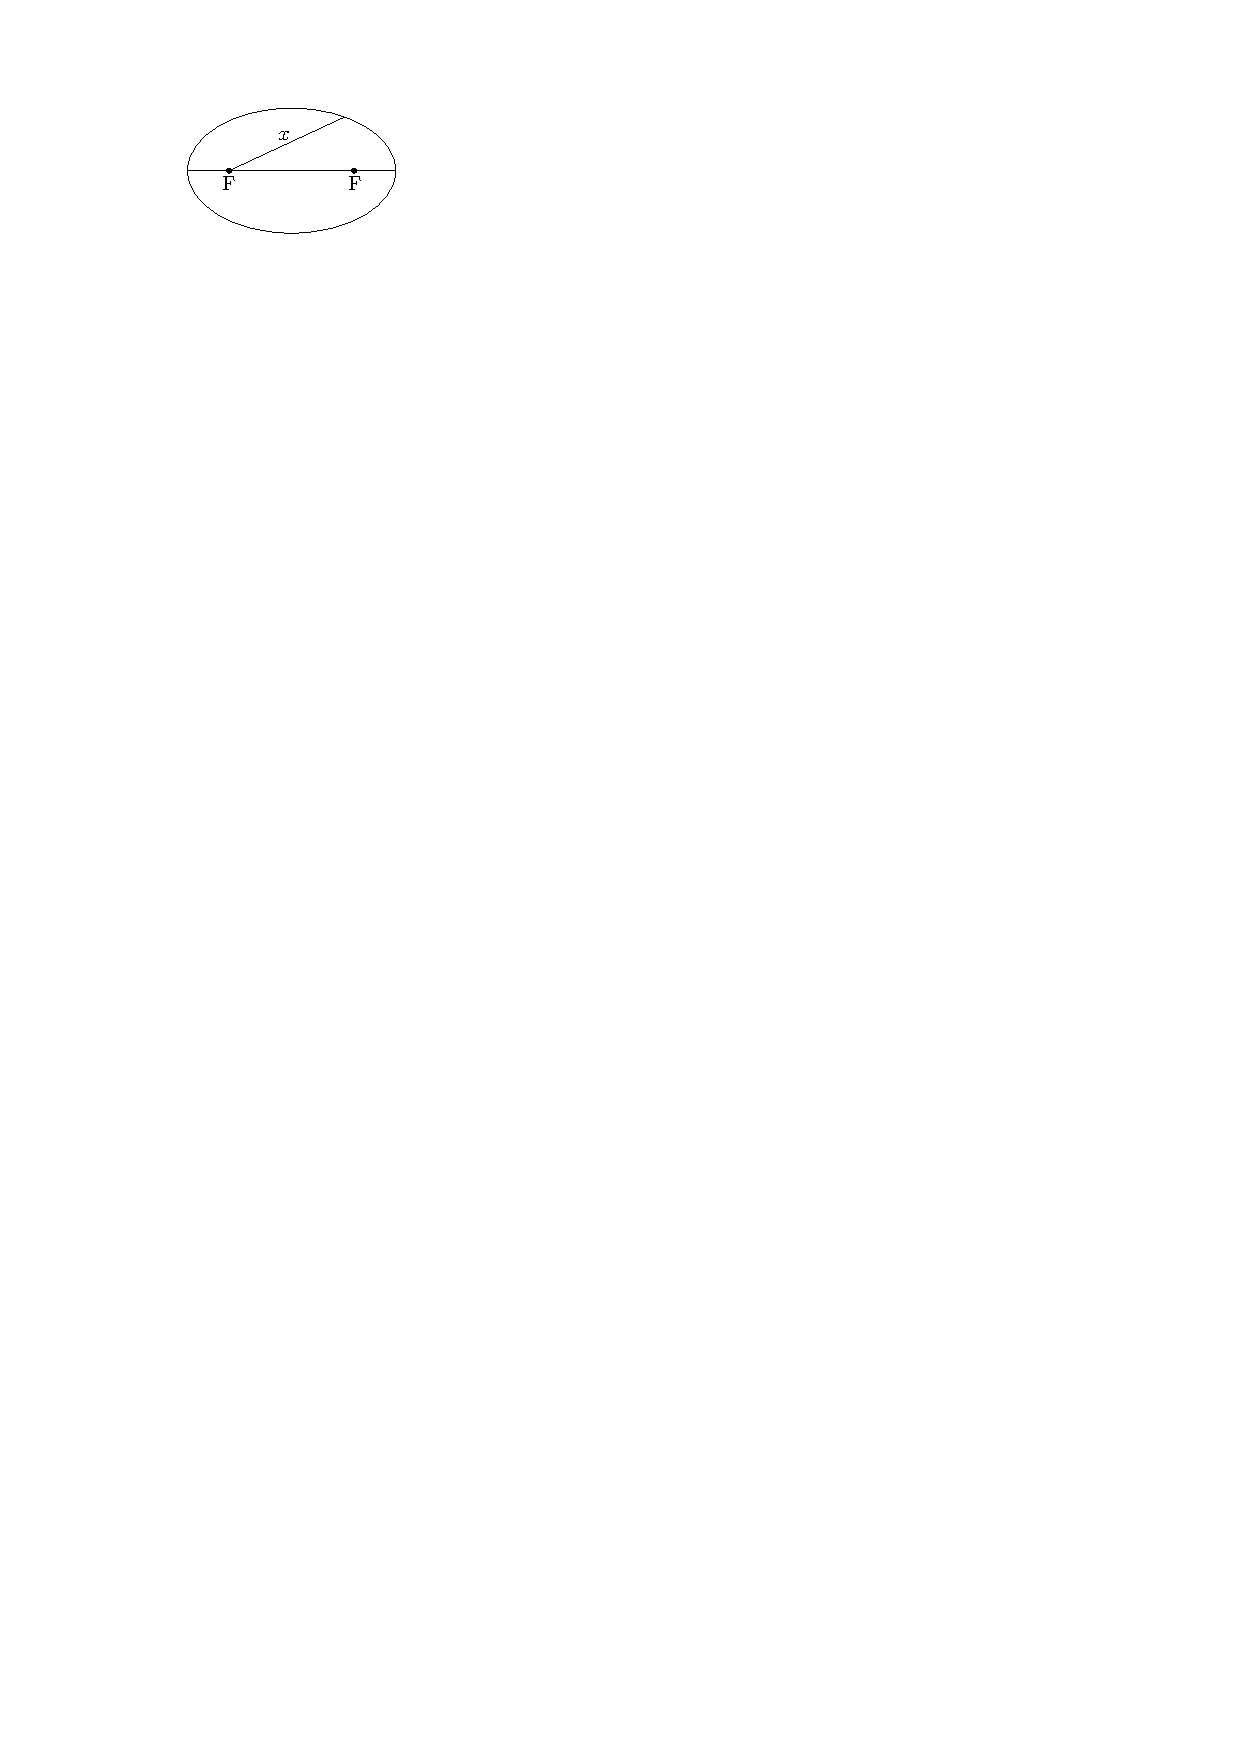
\includegraphics[width = 0.3\textwidth]{rad-curv}
\begin{figure}[!h]
\caption{К вычислению радиуса кривизны эллипса}
\end{figure}
\end{center}
\paragraph{Уравнения эллипса}
\begin{flushleft}
Каноническое уравнение
\end{flushleft}

\begin{equation}
\frac{x^2}{a^2}+\frac{y^2}{b^2}=1
\end{equation}
Параметрическое уравнение
\begin{equation}
\left\{\begin{aligned}[lcl]
&x=a\cos \varphi\\
&y=b\sin \varphi\\
\end{aligned}
\right.
\end{equation}

Уравнение в полярных координатах, где $\varphi$ --- истинная аномалия. При положительном знаке перед $e$ второй фокус эллипса будет находится в точке $(0,2c)$, а при отрицательном --- в точке $(\pi,2c)$.
\begin{equation}
r=\frac{p}{1\pm e\cos\phi}
\end{equation}

\paragraph{Оптические свойства эллипса}
\begin{enumerate}
\item Свет от источника, находящегося в одном из фокусов, отражается эллипсом так, что отражённые лучи пересекутся во втором фокусе.
\item Касательная эллипса образует с фокальными радиусами в точке касания равные острые углы.
\end{enumerate}





 
